\documentclass[11pt]{article}
\usepackage[margin=1in]{geometry}
\usepackage[T1]{fontenc}
\usepackage{lmodern}
\usepackage{microtype}
\usepackage{amsmath,amssymb,bm}
\usepackage{booktabs,tabularx,array}
\usepackage{xcolor}
\usepackage{tikz}
\usetikzlibrary{arrows.meta,calc,positioning,angles,quotes,patterns,decorations.pathreplacing}
\usepackage[colorlinks=true,allcolors=blue!55!black]{hyperref}
\usepackage[nameinlink,capitalise]{cleveref}
\usepackage[numbers,sort&compress]{natbib}

\title{Dislocation Loop Character in Irradiated Zirconium}
\author{}
\date{}

\newcommand{\hkil}[4]{[#1\,#2\,#3\,#4]}
\newcommand{\hkilp}[4]{(#1\,#2\,#3\,#4)}
\newcommand{\hkilf}[4]{\{#1\,#2\,#3\,#4\}}
\newcommand{\hkilfam}[4]{\langle #1\,#2\,#3\,#4\rangle}
\newcommand{\bvec}{\bm b}
\newcommand{\nvec}{\bm n}
\newcommand{\SI}[2]{\ensuremath{#1\,#2}}
\newcommand{\angstrom}{\mathring{\mathrm A}}
\newcommand{\meter}{\mathrm{m}}
\newcommand{\nano}{\mathrm{n}}
\newcommand{\celsius}{^{\circ}\mathrm{C}}
\newcommand{\kelvin}{\mathrm{K}}

\begin{document}
\maketitle

\begin{abstract}
Neutron, proton, electron, and heavy-ion irradiation of $\alpha$-zirconium and its alloys produces two principal families of dislocation loops: prismatic $\langle a\rangle$ loops with Burgers vector $\bvec=\tfrac13\langle11\bar20\rangle$, and basal $c$-component vacancy loops, most commonly faulted loops with $\bvec=\tfrac16\langle20\bar23\rangle$. This note summarizes their experimentally established character, crystallographic geometry, defect content, and dose--temperature regimes. Particular attention is given to the elliptical shape of $\langle a\rangle$ loops. The experimental difference between strongly elliptical vacancy loops and nearly circular interstitial loops is reconciled by combining equilibrium line-energy anisotropy with anisotropic point-defect transport.
\end{abstract}

\section{Crystallographic conventions}

At reactor-relevant temperatures zirconium is hexagonal close packed (HCP), with representative room-temperature lattice parameters
\begin{equation}
 a\simeq \SI{3.23}{\angstrom},\qquad c\simeq \SI{5.15}{\angstrom},
 \qquad c/a\simeq1.593.
\end{equation}
The basal plane is $(0001)$ and the $c$ axis is $[0001]$. The first- and second-order prismatic families are $\{10\bar10\}$ and $\{11\bar20\}$, respectively. A \emph{loop plane} or \emph{habit plane} is the plane containing the closed dislocation line. The Burgers vector does not, in general, uniquely determine that plane. A pure edge prismatic loop satisfies $\bvec\parallel\nvec$, but many experimentally observed $a$-loops are sheared or non-edge loops whose normals are tilted from this ideal orientation \citep{Jostsons1977Nature,Northwood1979RoundRobin}.

The HCP atomic volume is
\begin{equation}
 \Omega_{\rm Zr}=\frac{\sqrt3}{4}a^2c\simeq
 \SI{23.3}{\angstrom^3}=\SI{2.33e-29}{\meter^3}\quad\text{per atom}.
 \label{eq:atomic-volume}
\end{equation}
For a planar loop of area $A$, the signed number of point defects represented by its relaxation volume is approximately
\begin{equation}
 N=\frac{A\,\bvec\!\cdot\!\nvec}{\Omega_{\rm Zr}},
 \label{eq:defect-number}
\end{equation}
with the sign selected according to the line-sense convention; the magnitude distinguishes an interstitial platelet from a vacancy platelet.

\section{Experimentally observed loop families}

\subsection{Prismatic $\langle a\rangle$ loops}

The dominant loops at relatively low and intermediate irradiation exposure have
\begin{equation}
 \bvec_a=\frac13\langle11\bar20\rangle,
 \qquad |\bvec_a|=a\simeq\SI{0.323}{\nano\meter}.
 \label{eq:a-burgers}
\end{equation}
They contain no $c$ component and occur with both interstitial and vacancy character. At temperatures below approximately \SI{300}{\celsius}, the resolved $a$-loop population is commonly dominated by interstitial loops, although mixed populations are well documented and depend on temperature, dose, alloy chemistry, and irradiation spectrum \citep{Jostsons1977Nature,Northwood1979RoundRobin,Liu2020Platelets}.

The loop line lies on or near a prismatic plane. For example, a loop on $(10\bar10)$ lies in the plane spanned by $[0001]$ and the basal direction $[1\bar210]$. A second-order prismatic loop lies on a member of $\{11\bar20\}$. Experimental loop normals are distributed around these ideal prism orientations and may be tilted by up to roughly $30^\circ$, showing that many visible loops are not perfect edge loops \citep{Jostsons1977Nature,Northwood1979RoundRobin}.

The experimentally observed ellipse has
\begin{equation}
 \bm e_{\rm major}\approx[0001],\qquad
 \bm e_{\rm minor}\parallel(0001)\cap P_{\rm prism}.
 \label{eq:a-axes}
\end{equation}
Thus the long axis is approximately parallel to the $c$ axis, whereas the short axis is an $a$ direction lying in both the basal plane and the selected prismatic habit plane. This geometry is shown in \cref{fig:a-loop}.

\begin{figure}[htbp]
\centering
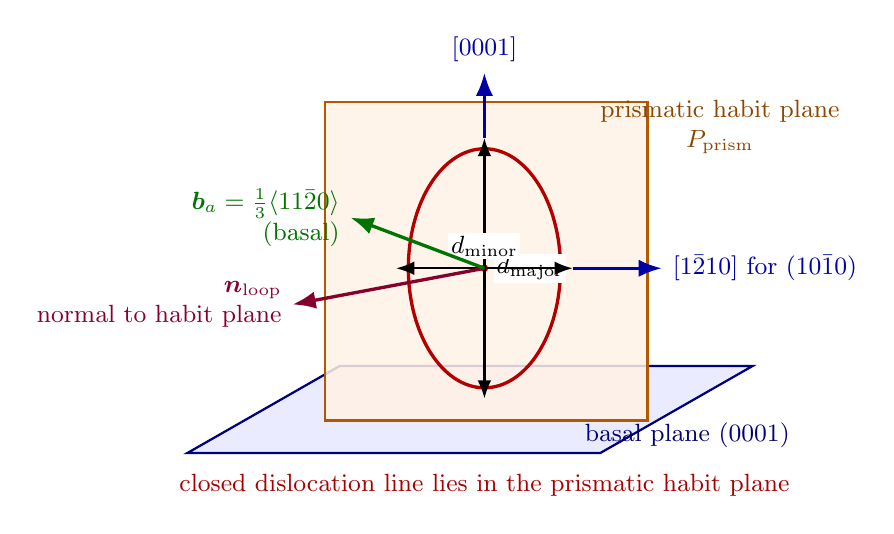
\begin{tikzpicture}[scale=0.92,>=Latex,font=\small]
  % basal plane
  \fill[blue!8] (-4,-2.0) -- (1.7,-2.0) -- (3.8,-0.8) -- (-1.9,-0.8) -- cycle;
  \draw[blue!50!black,thick] (-4,-2.0) -- (1.7,-2.0) -- (3.8,-0.8) -- (-1.9,-0.8) -- cycle;
  \node[blue!45!black] at (2.9,-1.75) {basal plane $(0001)$};
  % prism plane
  \fill[orange!10,opacity=.85] (-2.1,-1.55) -- (2.35,-1.55) -- (2.35,2.85) -- (-2.1,2.85) -- cycle;
  \draw[orange!70!black,thick] (-2.1,-1.55) rectangle (2.35,2.85);
  \node[orange!55!black,align=center] at (3.35,2.5) {prismatic habit plane\\$P_{\rm prism}$};
  % ellipse
  \draw[very thick,red!70!black] (0.1,0.55) ellipse [x radius=1.05,y radius=1.65];
  \fill[red!70!black] (0.1,0.55) circle (1.5pt);
  % axes
  \draw[<->,thick] (0.1,-1.25) -- (0.1,2.35)
    node[midway,right=3pt,fill=white,inner sep=1pt] {$d_{\rm major}$};
  \draw[<->,thick] (-1.12,0.55) -- (1.32,0.55)
    node[midway,above=3pt,fill=white,inner sep=1pt] {$d_{\rm minor}$};
  \draw[->,very thick,blue!65!black] (0.1,2.35) -- (0.1,3.25) node[above] {$[0001]$};
  \draw[->,very thick,blue!65!black] (1.32,0.55) -- (2.55,0.55)
    node[right] {$[1\bar210]$ for $(10\bar10)$};
  % normal
  \draw[->,very thick,purple!70!black] (0.1,0.55) -- (-2.55,0.05)
    node[left,align=right] {$\nvec_{\rm loop}$\\normal to habit plane};
  % b schematic
  \draw[->,very thick,green!45!black] (0.1,0.55) -- (-1.75,1.25)
    node[left,align=right] {$\bvec_a=\tfrac13\langle11\bar20\rangle$\\(basal)};
  \node[red!65!black] at (0.1,-2.45) {closed dislocation line lies in the prismatic habit plane};
\end{tikzpicture}
\caption{Geometry of an elliptical prismatic $a$-loop. The perspective drawing is schematic rather than metrically crystallographic. The loop plane contains $[0001]$ and one basal $a$ direction. The major axis is close to $[0001]$ and the minor axis lies in the basal plane. The Burgers vector is basal, while the measured habit-plane normal need not be exactly parallel to it.}
\label{fig:a-loop}
\end{figure}

\subsection{Basal $c$-component vacancy loops}

At higher exposure, vacancy loops with a $c$ component appear on basal planes. Their emergence correlates with accelerated or ``breakaway'' irradiation growth in many zirconium alloys \citep{Griffiths1987Neutron,Harte2017Matrix}. Several crystallographic states must be distinguished:
\begin{align}
 \bvec_{c/2}&=\frac12[0001], & |\bvec_{c/2}|&=\frac c2\simeq\SI{0.257}{\nano\meter},
 \label{eq:c2}\\
 \bvec_{c/2+p}&=\frac16\langle20\bar23\rangle,
 & |\bvec_{c/2+p}|&=\sqrt{\frac{a^2}{3}+\frac{c^2}{4}}
 \simeq\SI{0.318}{\nano\meter},
 \label{eq:c2p}\\
 \bvec_c&=[0001], & |\bvec_c|&=c\simeq\SI{0.515}{\nano\meter}.
 \label{eq:cfull}
\end{align}
The $c/2$ loop bounds a high-energy or extrinsic basal fault. Basal shear by a partial $\bm p=\tfrac13\langle1\bar100\rangle$ produces the commonly observed faulted $c/2+p$ loop,
\begin{equation}
 \frac12[0001]+\frac13\langle1\bar100\rangle
 =\frac16\langle20\bar23\rangle.
\end{equation}
The full-$c$ loop is unfaulted and may form by adding a second vacancy layer or by coalescence/reaction of suitable faulted loops \citep{Griffiths1987Neutron,Hulse2021Atomistic,Varvenne2014Vacancy}.

For all these basal loops,
\begin{equation}
 P_{\rm loop}=(0001),\qquad \nvec_{\rm loop}\parallel[0001].
 \label{eq:c-geometry}
\end{equation}
The entire closed dislocation line and both geometrical axes lie in the basal plane; the $c$ axis is normal to the loop. An isolated basal loop is often approximately circular because the basal plane has sixfold symmetry. If interactions, pinning, chemistry, stress, or coalescence produce an ellipse, both its major and minor axes remain basal directions; there is no universal in-plane major-axis direction. Recent high-burnup observations indeed show that some large $c$-component loops can be strongly noncircular \citep{Mayweg2024Islands}.

\begin{figure}[htbp]
\centering
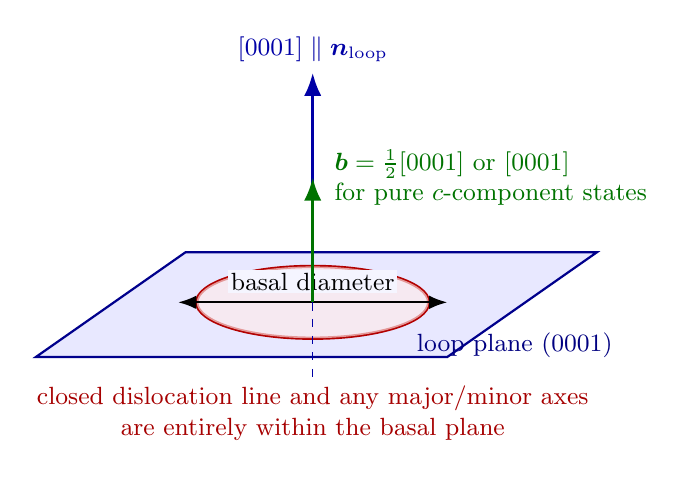
\begin{tikzpicture}[scale=0.95,>=Latex,font=\small]
  \fill[blue!9] (-3.7,-1.35) -- (1.8,-1.35) -- (3.8,0.05) -- (-1.7,0.05) -- cycle;
  \draw[blue!55!black,thick] (-3.7,-1.35) -- (1.8,-1.35) -- (3.8,0.05) -- (-1.7,0.05) -- cycle;
  \draw[very thick,red!70!black] (0,-0.62) ellipse [x radius=1.55,y radius=.48];
  \fill[red!8,opacity=.65] (0,-0.62) ellipse [x radius=1.55,y radius=.48];
  \draw[<->,thick] (-1.8,-0.62)--(1.8,-0.62)
    node[midway,above=3pt,fill=blue!4,inner sep=1pt] {basal diameter};
  \draw[->,very thick,blue!65!black] (0,-0.62)--(0,2.45)
    node[above] {$[0001]\parallel\nvec_{\rm loop}$};
  \draw[dashed,blue!65!black] (0,-0.62)--(0,-1.65);
  \draw[->,very thick,green!45!black] (0,-0.62)--(0,1.05)
    node[right=4pt,align=left] {$\bvec=\tfrac12[0001]$ or $[0001]$\\for pure $c$-component states};
  \node[blue!50!black] at (2.7,-1.2) {loop plane $(0001)$};
  \node[red!65!black,align=center] at (0,-2.1) {closed dislocation line and any major/minor axes\\are entirely within the basal plane};
\end{tikzpicture}
\caption{Geometry of a basal $c$-component vacancy loop. The apparent ellipse in this perspective drawing represents a circular basal loop viewed obliquely; it should not be interpreted as intrinsic ellipticity. For the faulted $c/2+p$ state, $\bvec$ additionally contains a basal partial component.}
\label{fig:c-loop}
\end{figure}

\begin{table}[htbp]
\centering
\caption{Principal irradiation-induced loop types in $\alpha$-Zr and zirconium alloys.}
\label{tab:loop-types}
\begin{tabularx}{\textwidth}{@{}l l l l X@{}}
\toprule
Type & Burgers vector & Habit plane & Character & Typical geometry and regime \\
\midrule
$a$ loop & $\tfrac13\langle11\bar20\rangle$ & near $\{10\bar10\}$ or $\{11\bar20\}$ & interstitial or vacancy & Appears early; generally elliptical, with major axis near $[0001]$ and minor axis basal. \\
$c/2$ loop & $\tfrac12[0001]$ & $(0001)$ & vacancy & Faulted basal precursor; pure-edge geometry when $\bvec\parallel\nvec$. \\
$c/2+p$ loop & $\tfrac16\langle20\bar23\rangle$ & $(0001)$ & predominantly vacancy & Common experimentally resolved basal faulted loop; appears at higher dose and is often large. \\
Full-$c$ loop & $[0001]$ & $(0001)$ & vacancy & Unfaulted, double-layer vacancy loop; less commonly identified. \\
\bottomrule
\end{tabularx}
\end{table}

\section{Ellipticity of prismatic $a$-loops}

\subsection{Experimental observations}

Let $d_{\max}$ and $d_{\min}$ denote the true major and minor diameters in the loop plane, and define
\begin{equation}
 e=1-\frac{d_{\min}}{d_{\max}}.
 \label{eq:ellipticity}
\end{equation}
Thus $e=0$ is circular. In the classic TEM measurements of neutron-irradiated high-purity Zr, $a$-loops were non-edge and elliptical, with the major axis near $[0001]$ \citep{Jostsons1977Nature}. The main quantitative trends were:
\begin{itemize}
 \item Interstitial $a$-loops became only mildly elliptical and reached approximately $e\simeq0.1$ for diameters above about \SI{20}{\nano\meter}. This corresponds to $d_{\max}/d_{\min}\simeq1.11$.
 \item Vacancy $a$-loops became increasingly elliptical with size and approached $e\simeq0.4$ near \SI{100}{\nano\meter}. This corresponds to $d_{\max}/d_{\min}\simeq1.67$.
\end{itemize}
The measurements exhibit substantial scatter. Reported image aspect ratios must also be corrected for projection if the loop plane is not normal to the electron beam. A circular inclined loop produces an elliptical TEM projection, so crystallographic tilting and habit-plane determination are essential before attributing the image shape to intrinsic ellipticity.

\subsection{Static energetic origin: anisotropic line tension}

For a loop of fixed area $A$, a circular shape minimizes perimeter only if the line energy $\lambda(\xi)$ is isotropic. Here $\xi$ denotes the local line direction. In HCP Zr, elastic anisotropy and orientation-dependent core structure make $\lambda$ different for segments parallel to basal directions and to $[0001]$. A convenient rectangular/elliptical approximation writes the line contribution as
\begin{equation}
 E_{\rm line}\sim L_a\lambda_a+L_c\lambda_c,
 \qquad \lambda_a>\lambda_c,
 \label{eq:line-energy}
\end{equation}
where $L_a$ and $L_c$ collect line segments of the corresponding orientations. The equilibrium Wulff-like shape sacrifices additional perimeter in order to reduce the total length weighted by high line energy. This produces elongation approximately along $[0001]$.

Atomistic calculations find representative ratios $\lambda_a/\lambda_c\simeq1.1$--$1.3$ for large $a$-loops \citep{Hulse2021Atomistic}. They predict that ellipticity increases with loop size: strongly overlapping strain fields and cores make very small loops nearly circular, whereas separated opposing segments in larger loops approach the anisotropic-line-tension limit. Importantly, static calculations predict similar optimum ellipticity for vacancy and interstitial loops. Typical predictions are $e\sim0$--$0.1$ for first-order prismatic loops and approximately $0.1$--$0.2$ for second-order prismatic loops over diameters of about 5--\SI{110}{\nano\meter}. Static energetics therefore explains moderate ellipticity and its size dependence, but not the much larger vacancy/interstitial difference observed experimentally.

\subsection{Kinetic origin: diffusional anisotropy difference}

Irradiation maintains nonequilibrium vacancy and SIA populations. Their diffusion tensors differ in HCP Zr; SIAs migrate particularly strongly in basal directions, while vacancy migration is generally less anisotropic and is sensitive to alloy chemistry and temperature \citep{Frank1988Defects,Woo1988Theory,Christiaen2021Influence}. Consequently, differently oriented portions of a prismatic loop do not receive identical point-defect fluxes.

Woo's diffusional-anisotropy-difference (DAD) model predicts that this kinetic contribution changes the two loop characters in opposite directions \citep{Woo1988Theory}:
\begin{equation}
 \text{line/core anisotropy}
 \quad+\quad
 \begin{cases}
   \text{DAD increases ellipticity}, & \text{vacancy }a\text{-loop},\\
   \text{DAD decreases ellipticity}, & \text{interstitial }a\text{-loop}.
 \end{cases}
 \label{eq:reconciliation}
\end{equation}
The combined model reconciles the evidence. Static anisotropic line energy gives both characters a moderate tendency toward the same elongated shape. Irradiation-driven anisotropic absorption then amplifies that tendency for vacancy loops and suppresses it for interstitial loops. The result is consistent with $e_{\rm vac}\simeq0.4$ but $e_{\rm int}\simeq0.1$ at sufficiently large size.

\begin{figure}[htbp]
\centering
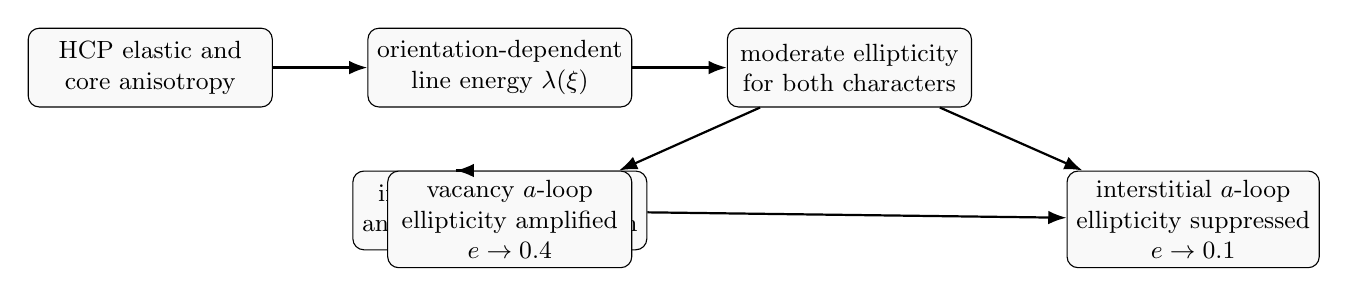
\begin{tikzpicture}[>=Latex,font=\small,node distance=8mm and 12mm]
 \tikzset{box/.style={draw,rounded corners,align=center,minimum height=10mm,minimum width=31mm,fill=gray!5},
          arr/.style={->,thick}}
 \node[box] (hcp) {HCP elastic and\\core anisotropy};
 \node[box,right=of hcp] (static) {orientation-dependent\\line energy $\lambda(\xi)$};
 \node[box,right=of static] (base) {moderate ellipticity\\for both characters};
 \draw[arr] (hcp)--(static); \draw[arr] (static)--(base);
 \node[box,below=of static] (flux) {irradiation defect flux\\and anisotropic diffusion};
 \node[box,below left=of base] (vac) {vacancy $a$-loop\\ellipticity amplified\\$e\rightarrow0.4$};
 \node[box,below right=of base] (sia) {interstitial $a$-loop\\ellipticity suppressed\\$e\rightarrow0.1$};
 \draw[arr] (flux)--(vac); \draw[arr] (flux)--(sia);
 \draw[arr] (base)--(vac); \draw[arr] (base)--(sia);
\end{tikzpicture}
\caption{Reconciliation of equilibrium and kinetic explanations for $a$-loop ellipticity. The numerical limiting values summarize the classic large-loop TEM observations and should not be treated as universal constants for every alloy and irradiation condition.}
\label{fig:ellipticity-model}
\end{figure}

\subsection{Dependence on irradiation conditions and alloy state}

Ellipticity is most evident for resolvable prismatic $a$-loops that have grown beyond the small-cluster regime. Temperature must be high enough for point-defect migration and loop growth, while sustained irradiation supplies the flux needed for DAD to modify the static shape. The classic quantitative observations were obtained in neutron-irradiated Zr at approximately \SI{668}{\kelvin}, with mixed interstitial/vacancy populations \citep{Jostsons1977Nature}. The shape is not controlled by dose or temperature alone: size, habit plane, loop character, diffusion tensor, and local pinning must all be considered.

Alloying and irradiation-induced segregation can change point-defect mobilities, core energies, and local stresses. Fe, Ni, Cr, and Sn redistribution near loop arrays has been observed in irradiated Zircaloy-2 \citep{Harte2017Matrix}. Solute atmospheres, second-phase particles, other loops, free surfaces, and network dislocations can pin selected line segments and produce shapes that depart from a smooth equilibrium ellipse. Hence the aspect ratios above are useful benchmark values, not universal constitutive constants.

\section{Why basal $c$-component loops are usually more nearly circular}

For an isolated loop in $(0001)$, the sixfold basal symmetry makes the in-plane line-energy variation much smaller than that experienced around a prismatic $a$-loop. Earlier TEM studies therefore commonly described faulted $c/2+p$ loops as circular or nearly circular \citep{Harte2017Matrix,Hulse2021Atomistic}. Their geometry is also fundamentally different: the $[0001]$ direction is the loop normal, not an in-plane major axis.

Large high-dose $c$-component loops need not remain circular. Local stress, anisotropic segregation, interaction and coalescence, crystallographic faceting, or pinning can break the nominal basal symmetry. Recent high-burnup cladding examinations report strongly noncircular $c$-loops and chemical partitioning at and inside them \citep{Mayweg2024Islands}. A universal experimental aspect ratio has not yet emerged for this newer class of observations. Any model that assigns ellipticity to basal loops should therefore specify the symmetry-breaking field or kinetic mechanism instead of transferring the well-established prismatic $a$-loop aspect ratios to $c$-loops.

\section{Summary}

\begin{enumerate}
 \item $a$-loops have $\bvec=\tfrac13\langle11\bar20\rangle$, occur with both vacancy and interstitial character, and lie on or near prismatic planes. Their major axis is near $[0001]$ and their minor axis is the basal direction contained in the habit plane.
 \item Basal $c$-component loops are predominantly vacancy loops. The common faulted state has $\bvec=\tfrac16\langle20\bar23\rangle$; $c/2$ and full-$c$ states are also possible. Their loop line and both shape axes lie in $(0001)$, while $[0001]$ is normal to the loop.
 \item Large vacancy $a$-loops reach approximately $e\simeq0.4$ ($d_{\max}/d_{\min}\simeq1.67$), whereas interstitial $a$-loops plateau near $e\simeq0.1$ ($d_{\max}/d_{\min}\simeq1.11$) in the classic experiments.
 \item Anisotropic elastic/core line energy explains moderate ellipticity and its increase with loop size. Diffusional anisotropy under irradiation amplifies vacancy-loop ellipticity and suppresses interstitial-loop ellipticity, reconciling static models with TEM observations.
\end{enumerate}

\bibliographystyle{unsrtnat}
\bibliography{Loop_character}

\end{document}